\documentclass[11pt,a4paper]{article}
\usepackage[T1]{fontenc}
\usepackage[utf8]{inputenc}
\usepackage{lmodern}
\usepackage[margin=25mm]{geometry}
\usepackage{amsmath,amssymb,booktabs,longtable,array,graphicx}
\usepackage[numbers,sort&compress]{natbib}
\usepackage{microtype}
\usepackage[hidelinks]{hyperref}
\usepackage{placeins}
\setlength{\emergencystretch}{2em}
\title{Regularization and Observation Timing in Joint Heat Diffusivity and Initial-State Recovery: A Controlled PINN Audit}
\author{Ridoy Hasan\\Comilla University, Cumilla, Bangladesh\\
\href{mailto:hasanridoy@stud.cou.ac.bd}{\texttt{hasanridoy@stud.cou.ac.bd}}}
\date{}
\begin{document}
\maketitle
\begin{abstract}
Estimating thermal diffusivity from sparse temperature measurements becomes harder when the initial temperature is unknown. This study examines whether apparent advantages of a physics-informed neural network (PINN) persist against regularized spectral inversion, and how observation timing changes the comparison. A one-dimensional synthetic heat problem is studied in stages: an original comparison with 400 pipeline jobs, a paired timing evaluation with 360 datasets and 720 fits, and a localized off-basis evaluation with 120 datasets and 240 fits. Separate post-evaluation analyses examine profiled objectives, matrix rank, initial-state flexibility, and independent propagation of recovered PINN quantities. In the original comparison, the longer-budget PINN had lower diffusivity error than cross-validated twelve-mode inversion in nine of ten sparse designs for the richer initial field. The prespecified timing interaction for that field with ten observations was 3.7322 percentage points, with a 95\% percentile bootstrap interval of $[-0.0947,56.2421]$, leaving its direction unresolved. Twelve unrestricted initial coefficients could locally interpolate ten observations across diffusivities whenever the observation matrix had full row rank. Independent propagation exposed network--solution discrepancies up to 11.65\%. The localized field extended the comparison beyond finite twelve-mode truths, but changed signal energy as well as representation mismatch. The findings support conditional comparisons of specified estimators, not universal method superiority or restored unconstrained identifiability.
\end{abstract}
\noindent\textbf{Keywords:} inverse heat conduction; physics-informed neural networks; regularization; observation timing; initial-state recovery; identifiability.

\section{Introduction}
Temperature measurements contain information about both how quickly heat spreads and how it was distributed initially. If the starting temperature is known, an inverse method can adjust diffusivity to explain later measurements. If the starting temperature is unknown, changing that field can also explain changes in the observations. Accurate interpolation of a few measurements is therefore not sufficient evidence that the inferred diffusivity or initial field is correct.

The underlying inverse problem is established. Scarpa and Tagliafico examined the effect of biased initial temperature on thermophysical-property estimation and included initial-temperature parameters in an estimation procedure \citep{scarpa2015}. Zhao and colleagues studied simultaneous recovery of diffusivity and initial state, including source recovery and boundary-control formulations \citep{ref002,ref003}. Their measurement and excitation conditions differ from finite, noisy interior samples with homogeneous boundary values. More generally, regularization is essential when discrete inverse problems admit unstable or nonunique reconstructions \citep{ref010,ref011}. The present setting instead uses a fixed number of noisy interior measurements without controlled boundary excitation.

Physics-informed neural networks combine observation fitting with differential-equation residuals \citep{ref001,ref031}. Their use for noisy inverse problems includes Bayesian formulations \citep{ref038} and application-specific comparisons with classical methods. Zapf and colleagues compared neural and finite-element approaches to diffusivity estimation from brain tracer images \citep{ref006}. Grossmann and colleagues compared PINNs and finite elements for forward problems \citep{ref005}. Jekic and colleagues studied noisy inverse fluid problems with a finite-element/optimization reference and prescribed initial-condition data \citep{ref096}. Zhang, Alla and Karniadakis explicitly examined comparison controls in adjoint and PINN inverse procedures \citep{zhang2026}. Oliveira and colleagues investigated reconstruction of initial temperature for heat problems with specified diffusivity \citep{ref004}. These studies motivate controlling both the classical reference and the initial-state information available to the methods.

Identifiability with an unknown initial field also has close precedents. Salmaniw and Browning connect initial conditions to identifiability in parabolic equations and profile unknown initial-state coefficients in a practical reaction--diffusion example \citep{ref076}. Their structural analysis assumes full observation; their practical example jointly estimates diffusion and reaction rates. BiLO includes heat initial-state recovery with fixed diffusivity and compares it with a PINN approach \citep{bilo2026}. Here diffusivity and the initial field are both unknown, and the comparison uses sparse interior measurements with paired timing schedules and observation-based regularization selection.

The question here is narrower: when diffusivity and initial temperature are both unknown, how does the comparison between specified PINN and cross-validated spectral procedures depend on regularization, initial-state representation, optimization budget, and measurement schedule? This computational audit uses synthetic observations to connect paired method comparisons with checks of the information supplied by the data, the restrictions imposed by the initial-state representation, and the physical consistency of the learned quantities.

The experiments were conducted in stages. The original comparison tested regularization, six- versus twelve-mode classical representations, and two neural budgets. A separately frozen follow-up compared early, mixed, and late observations at fixed measurement count and absolute noise level. Post-evaluation diagnostics then examined coefficient-profiled objectives, conditioning, basis flexibility, and independent heat propagation. A further frozen evaluation tested one localized initial field outside the twelve-mode span. Each stage retains its own sampling unit and estimator definition. Their run counts are not pooled into an enlarged independent sample.

\section{Problem and experimental design}
\subsection{Heat model and observations}
The normalized model is
\begin{equation}
 u_t=\alpha u_{xx},\quad (x,t)\in(0,1)\times(0,1],\qquad
 u(0,t)=u(1,t)=0,\quad u(x,0)=f(x).
\label{eq:heat}
\end{equation}
Both the constant diffusivity $\alpha$ and the initial field $f$ are unknown to the estimators. The geometry and boundary values are known. This benchmark does not assign a specific physical material or experimental units. The true diffusivity is $\alpha^*=0.05$, and the first two initial fields are
\begin{equation}
 f_A(x)=\sin(\pi x)+0.5\sin(3\pi x),\qquad
 f_B(x)=f_A(x)+0.25\sin(7\pi x).
\end{equation}
Their exact solutions follow by multiplying the coefficient of mode $j$ by $\exp[-\alpha^*(j\pi)^2t]$. Observations are
\begin{equation}
 y_i=u^*(x_i,t_i)+\sigma z_i,\qquad \sigma=0.01,\quad z_i\sim\mathcal N(0,1),
\end{equation}
with independent standard-normal draws within each design. Neither true coefficients nor initial-field measurements are given to either estimator. Noise is fixed in absolute temperature units, not as a fraction of the signal.

\subsection{Three evaluation stages}
Table~\ref{tab:design} distinguishes datasets, independent design/noise blocks, and pipeline jobs. A block contains the random spatial locations, base time draws, standardized noise, and validation-fold labels shared across the conditions specified within that stage. Development pilots are excluded from the evaluation summaries. The use of distinct stages follows the need to distinguish method development from performance evaluation \citep{ref068,ref080}.
\begin{table}[htbp]\centering\small
\caption{Evaluation structure. Block counts are totals across the two observation counts. A job is a reported procedure output or neural fit, not an independent experimental replicate.}\label{tab:design}
\begin{tabular}{lrrrp{53mm}}\toprule
Stage & Blocks & Datasets & Jobs & Procedures\\\midrule
Original comparison & 20 & 40 & 400 & Four spectral procedures; two PINN budgets, three starts each\\
Controlled timing & 60 & 360 & 720 & CV12 and one PINN-1000 start\\
Localized field & 60 & 120 & 240 & CV12 and one PINN-1000 start\\\bottomrule
\end{tabular}
\end{table}

In the original comparison, $N=10$ or $50$ points were sampled uniformly over the unit space--time square. There were ten independent blocks per observation count, shared across fields A and B. This gives 40 dataset cases but only 20 independent base blocks. Four spectral outputs and six neural fits were retained for each case.

The timing evaluation used 30 fresh blocks per observation count. For base draws $q_i\sim U(0,1)$, the early and late schedules were $t_i^{\mathrm{early}}=0.01+0.09q_i$ and $t_i^{\mathrm{late}}=0.20+0.60q_i$. A separate seeded random permutation assigned exactly half the indices to early times for the mixed schedule; the remainder used their late times. All three schedules shared the spatial coordinates, noise draws and folds, as did A and B. This produced $2\times2\times3\times30=360$ datasets. The schedules alter temporal spread as well as delay. Under fixed absolute noise, they also alter signal-to-noise ratio.

The off-basis evaluation used 30 further fresh blocks per observation count and only mixed and late schedules. Its initial field was
\begin{equation}
 f_C(x)=\frac{g(x)}{\max_{s\in[0,1]}g(s)},\qquad
 g(x)=x(1-x)\exp\left[-\frac{(x-0.35)^2}{2(0.04)^2}\right].
\label{eq:localized}
\end{equation}
This smooth, zero-boundary field has a localized warm region and is not a finite twelve-mode sine combination. Its reference evolution was verified by spectral refinement and an independent finite-difference calculation before inverse evaluation. The same diffusivity, absolute noise, estimator bounds and retained pilot fitting settings were used. This stage contains 120 datasets, with schedules paired within each block.

\section{Inverse procedures and analysis}
\subsection{Classical spectral inversion}
For a basis size $M$, the classical field is
\begin{equation}
 \widehat u_M(x,t)=\sum_{j=1}^{M} a_j\sin(j\pi x)e^{-\alpha(j\pi)^2t}.
\end{equation}
It satisfies Equation~\eqref{eq:heat} exactly for the fitted $\alpha$. At each candidate diffusivity, coefficients minimize
\begin{equation}
 J_{M,\lambda}(\alpha,\boldsymbol a)
 =\frac{1}{N}\|B(\alpha)\boldsymbol a-\boldsymbol y\|_2^2
 +\lambda\sum_{j=1}^{M}j^4a_j^2,
 \quad B_{ij}(\alpha)=\sin(j\pi x_i)e^{-\alpha(j\pi)^2t_i}.
\label{eq:ridge}
\end{equation}
Eliminating linear coefficients before searching nonlinear parameters is related to established variable-projection methods \citep{ref020,ref021}. Here augmented least squares computes the conditional coefficients without forming normal equations. Diffusivity is restricted to $[10^{-5},1]$. The search evaluates 1601 equally spaced log-diffusivity points, refines detected interior local minima by bounded scalar minimization with log-coordinate tolerance $10^{-11}$, and compares refined, grid and endpoint candidates. It is an extensive scalar search, not a certificate of global optimality.

The original procedures were unregularized six-mode inversion (unreg6), six-mode inversion with $\lambda=10^{-6}$ (fixed6), and cross-validated six- and twelve-mode inversion (CV6 and CV12). Five balanced folds selected $\lambda$ from $\{10^{-10},10^{-8},10^{-6},10^{-4},10^{-2}\}$. Each candidate was fitted on the training folds; selection minimized the pooled held-out squared error divided by $N$, with exact ties resolved toward the smaller penalty. The selected penalty was refitted using all observations. Synthetic truth did not enter selection.

The timing and localized-field stages retained CV12 and expanded the penalty grid to include $10^{-14}$ and $10^{-12}$ after separate development checks, before evaluation. This change prevents treating the stages as evaluations of an identical classical pipeline. Positive penalties give unique conditional coefficients but do not establish joint identifiability. The $j^4$ penalty favors smooth initial fields; changing basis size changes the procedure even when this formula is retained. Both A and B lie inside the twelve-mode representation, which advantages this classical reference relative to an unrestricted choice of true fields.

\subsection{PINN representation and optimization}
The neural field is $\widehat u_\theta(x,t)=x(1-x)g_\theta(x,t)$, enforcing the homogeneous boundary values exactly. Hard boundary constructions are established in neural PDE methods \citep{ref053}. The network has three hidden layers of 32 hyperbolic-tangent units and a linear scalar output. Inputs are scaled to $[-1,1]$; weights use Xavier-normal initialization with tanh gain and zero biases \citep{ref065}. An unconstrained scalar $r$ defines
\begin{equation}
 \alpha(r)=\exp\{\log(10^{-5})+[\log(1)-\log(10^{-5})]\operatorname{sigmoid}(r)\},
\end{equation}
initialized to $\alpha=0.2$. Unlike the classical endpoint search, this parameterization approaches its bounds continuously. No initial-condition loss or initial-temperature samples are supplied.

Training minimizes
\begin{equation}
 \mathcal L=\frac{10}{N}\sum_{i=1}^N[\widehat u_\theta(x_i,t_i)-y_i]^2
 +\frac{1}{512}\sum_{k=1}^{512}[\partial_t\widehat u_\theta-\alpha\partial_{xx}\widehat u_\theta]^2(x_k^c,t_k^c).
\end{equation}
Automatic differentiation computes derivatives \citep{ref066}. The 512 uniform collocation points, seed 314159, are fixed across fits. They are equation-enforcement points, not additional temperature measurements. Another 2048 points, seed 271828, are reserved for residual diagnostics. Their residuals neither select a fit nor replace recovery errors.

All neural fits use 2000 full-batch Adam steps \citep{ref060}, with learning rates 0.001 for weights and 0.01 for $r$, followed by L-BFGS \citep{ref061}. The original comparison retains caps of 200 or 1000 L-BFGS iterations (PINN-200 and PINN-1000), maximum evaluation settings of 250 or 1250, and initialization seeds 101, 102 and 103. L-BFGS uses learning rate 1, strong-Wolfe line search, history size 50, gradient tolerance $10^{-12}$ and change tolerance $10^{-14}$. A 600-second training limit is declared per fit. The follow-ups use PINN-1000 and the prespecified seed 101 only. There is no selection of the best initialization using truth.

Neural settings were retained from development rather than tuned by a search equivalent to classical cross-validation. Unequal tuning opportunities are therefore a limitation. Existing analyses of PINN training and inverse-error bounds also caution against equating low loss with accurate physical recovery without the required assumptions \citep{ref045,ref046,ref043}.

\subsection{Recovery errors, pairing and uncertainty}
The three reported errors are
\begin{equation}
 E_\alpha=100\frac{|\widehat\alpha-\alpha^*|}{\alpha^*},\quad
 E_f=100\frac{\|\widehat u(\cdot,0)-f\|_{L^2(0,1)}}{\|f\|_{L^2(0,1)}},\quad
 E_u=100\frac{\|\widehat u-u^*\|_{L^2((0,1)^2)}}{\|u^*\|_{L^2((0,1)^2)}}.
\end{equation}
Trapezoidal quadrature uses 401 spatial and temporal grid points, with planned 801-point checks on the first design of each stratum. Initial-field scoring for C compares directly with Equation~\eqref{eq:localized}. Observation coordinates, collocation points and scoring grids serve different roles.

In the original comparison, each neural dataset score is the median over three starts, separately for each outcome. Those outcome medians need not belong to one network; they describe initialization performance, not an ensemble or deployable selection rule. The follow-ups score the one declared start directly. Results are not pooled across these estimator definitions.

For each timing block $b$ and schedule $s$, define
\begin{equation}
 D_b(s)=E_{\alpha,b}^{\mathrm{PINN}}(s)-E_{\alpha,b}^{\mathrm{CV12}}(s),\qquad
 I_b=D_b(\mathrm{mixed})-D_b(\mathrm{late}).
\label{eq:interaction}
\end{equation}
The prespecified primary timing result is $\operatorname{median}_b I_b$ for $N=10$, field B. Negative $D$ indicates lower PINN error; positive $I$ indicates a larger PINN-minus-CV12 gap under mixed observations. Neither is obtained by subtracting marginal medians. Percentile bootstrap intervals use 10000 resamples of whole independent blocks \citep{ref081,ref083}; the timing primary seed is 908000. The original comparison uses ten blocks per stratum and the follow-ups use thirty. All other timing and localized-field intervals are pointwise secondary summaries, with no simultaneous-coverage claim. Skewed distributions, near-bound estimates and small block counts can make these intervals unstable. An interval spanning zero establishes neither equivalence nor absence of a timing effect.

Failures and interrupted fits were to be retained without replacement. Complete-block comparisons are conditional on the required estimates being available, and finite capped estimates remain included. Completed jobs need not have converged to accurate physical parameters. Dataset counts and optimizer runs should not be interpreted as counts of independent statistical tests.

\subsection{Post-evaluation identifiability and physical checks}
These analyses explain the frozen timing procedures; they were not prespecified primary tests. At each diffusivity, coefficients are fitted before plotting residual or penalized objective profiles. Singular values of $B(\alpha)$ give numerical rank with threshold $\max(N,M)\epsilon_{\mathrm{mach}}\sigma_1$. Raw residual profiles and coefficient norms complement penalized profiles. Different penalties define different objectives, so their vertical ordering is not a valid penalty-selection criterion or a confidence interval.

For $N=10$, $M=12$, if $B(\alpha)$ has full row rank, then
\begin{equation}
 \boldsymbol a(\alpha)=B(\alpha)^T[B(\alpha)B(\alpha)^T]^{-1}\boldsymbol y
\label{eq:interpolation}
\end{equation}
interpolates all observations in exact arithmetic. A nonzero full-rank minor remains nonzero in a neighborhood by continuity, so nearby diffusivities also interpolate with adjusted coefficients. Equation~\eqref{eq:interpolation} is an explanatory identity, not the numerical implementation. Ill-conditioning and large coefficient norms can limit its practical realization. This is standard linear algebra applied to this design, not a new identifiability theorem \citep{ref011}. Additional post-evaluation CV6 and CV24 fits use the expanded penalty grid, adding 720 fits across the 360 timing datasets. They assess sensitivity without replacing the original CV12 results.

For each of the 360 timing PINNs, an independent sine-series solver propagates the learned initial field $\widehat u_\theta(x,0)$ using the learned diffusivity. It does not use true parameters to construct the rollout. A discrete sine transform extracts coefficients; the initial comparison uses 256 modes from 2048 quadrature intervals and 512 modes from 4096 intervals. On the 401-by-401 grid, the discrepancy is
\begin{equation}
 C=100\frac{\|\widehat u_\theta-u_{\mathrm{rollout}}\|_{L^2((0,1)^2)}}{\|u_{\mathrm{rollout}}\|_{L^2((0,1)^2)}}.
\end{equation}
Relative forward refinement, initial reconstruction and change under a 201-point scoring grid are screened at $10^{-4}$ in ratio units. This is a numerical refinement screen, not a threshold for physical acceptability. One screened case was refined separately through 512, 1024 and 2048 modes. A small $C$ would establish consistency of learned quantities with the network trajectory, not accuracy of those quantities against truth.

\subsection{Reproducibility and chronology}
The original, timing and localized-field evaluations have separate prospective source and configuration freezes, development records and fresh seed sets. These are local versioned protocols, not formal preregistrations. Post-evaluation diagnostics and publication figures are labeled separately. The computations use CPU double precision; exact environment and threadpool metadata are archived with each run. The original evaluation recorded Python 3.14.6, NumPy 2.5.4 and PyTorch 2.15.0+cpu, with one-thread controls. Environment records, rather than a later software installation, specify how the saved experiments were run.

Saved observations, folds, classical candidates, neural checkpoints, traces, scoring checks and hash manifests allow inspection without repeating all optimization. The evidence release also supplies restoration instructions. Runtime measurements must be interpreted by their scope: original selection-plus-fit and neural-training timers exclude evaluation, whereas follow-up job timers include saved diagnostics and scoring. No equal-compute superiority is inferred from their comparison.

\section{Results}
\subsection{Original comparison: regularization, representation and budget}
All 400 scheduled jobs completed, comprising 160 reported classical outputs and 240 neural fits. They arose from 40 dataset cases sharing 20 independent base blocks. All neural fits reached their configured iteration caps; this is budget completion, not certified convergence. The planned scoring refinement checks changed full-field errors by at most 0.001868 percentage points and initial-field errors by approximately $7.04\times10^{-8}$ percentage points.

Regularization substantially changed the baseline in sparse field A. Median initial-field error was 37.274\% for unreg6, 8.508\% for fixed6 and CV6, and 10.900\% for CV12. The two PINN medians were 8.803\% and 8.963\%. Thus the apparent advantage over unregularized inversion was much less distinctive against regularized procedures. The full original table is retained in Appendix~\ref{app:original}.

For field B with ten observations, PINN-1000 had lower diffusivity and initial-field errors than CV12 in nine of ten designs each. Median paired differences were $-4.445$ percentage points for diffusivity, with pointwise 95\% interval $[-22.168,-1.109]$, and $-1.508$ for the initial field, with interval $[-5.148,-0.467]$. Full-field error was lower in eight designs. With fifty observations, CV12 had lower full-field error than PINN-1000 in eight designs; the PINN-minus-CV12 median difference was $+0.803$ percentage points, interval $[0.032,2.142]$. The corresponding diffusivity and initial-field intervals spanned zero. Figure~\ref{fig:original} retains all planned original contrasts, including uncertain comparisons.

The six-mode field cannot represent the seventh component in B. Orthogonality gives the initial-field relative error floor $100(0.25)/\sqrt{1+0.5^2+0.25^2}=21.82\%$. All sixty six-mode B outputs respected this floor. Twelve modes contain both truths, but added capacity did not uniformly improve sparse recovery. Longer neural optimization also had no uniform benefit: at $N=50$/A, median initial-field error increased from 1.573\% to 2.366\% between the two budgets; at $N=50$/B it decreased from 22.352\% to 16.482\%. These are descriptive patterns, not evidence that budget should be selected using recovery truth.

\begin{figure}[htbp]\centering
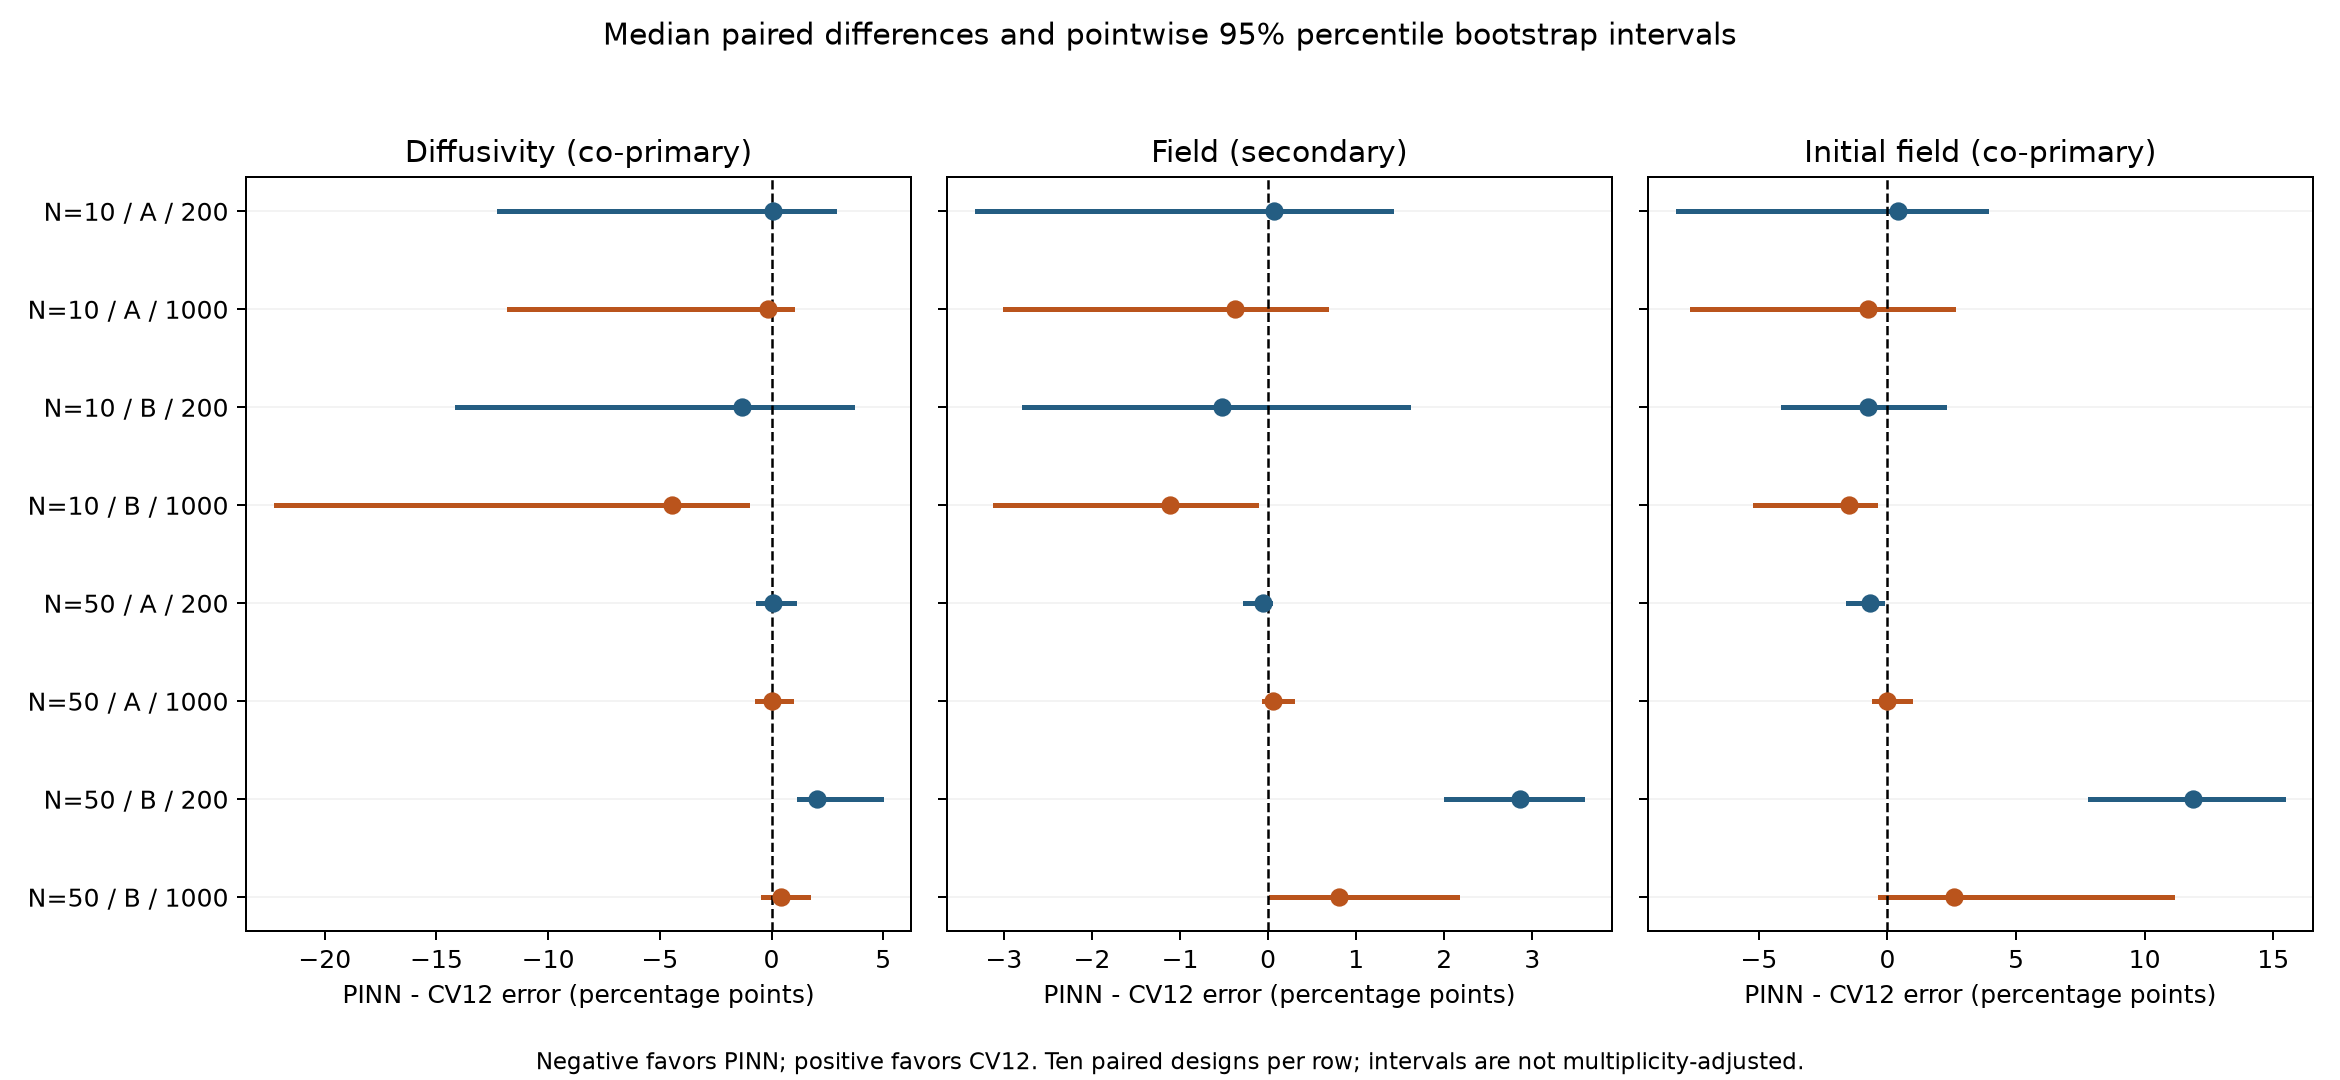
\includegraphics[width=\linewidth]{figures/original-paired.png}
\caption{Original comparison: all planned paired contrasts against CV12. Negative differences favor the PINN. Neural dataset scores are outcome-specific medians over three starts. Intervals are pointwise 95\% percentile intervals for median paired differences across ten independent designs per stratum; they are not simultaneous intervals.}\label{fig:original}
\end{figure}

\subsection{Controlled timing: the primary interaction remains uncertain}
All 720 fits completed across 360 datasets. Table~\ref{tab:timing} gives absolute diffusivity errors; Figure~\ref{fig:timing} displays the prespecified stratum and the blockwise interaction. For $N=10$/B, the median interaction was 3.7322 percentage points, with 95\% percentile interval $[-0.0947,56.2421]$. Its sign is unresolved. The interval permits a substantial positive interaction and does not demonstrate equivalence of the schedules.

\begin{table}[htbp]\centering\small
\caption{Timing evaluation: marginal median diffusivity errors (\%). Each row has thirty paired blocks. These are not paired effect estimates.}\label{tab:timing}
\begin{tabular}{rllrr}\toprule
$N$ & Field & Schedule & CV12 & PINN-1000\\\midrule
10 & A & early & 28.303 & 99.863\\
10 & A & mixed & 5.113 & 6.616\\
10 & A & late & 29.470 & 7.939\\
10 & B & early & 90.130 & 99.951\\
10 & B & mixed & 10.862 & 10.410\\
10 & B & late & 29.515 & 7.749\\
50 & A & early & 5.111 & 4.792\\
50 & A & mixed & 1.586 & 1.267\\
50 & A & late & 1.736 & 1.500\\
50 & B & early & 3.528 & 6.207\\
50 & B & mixed & 1.287 & 1.398\\
50 & B & late & 1.702 & 1.557\\
\bottomrule\end{tabular}
\end{table}


For that same stratum, the median paired diffusivity gap was $-0.047$ percentage points under mixed observations, with pointwise interval $[-1.516,1.195]$, and $-0.976$ under late observations, with interval $[-22.424,-0.066]$. The PINN had lower diffusivity error in 18 and 25 of 30 blocks, respectively. These secondary schedule contrasts do not supersede the primary interaction. Their paired medians differ markedly from the differences between marginal medians in Table~\ref{tab:timing}.

Both procedures performed poorly in many ten-observation early cases. CV12 returned lower-bound estimates in 44 of 360 timing fits. The original neural bound flag marked none, but the smallest neural estimate was $1.002115\times10^{-5}$, only about 0.211\% above the lower bound. For ten early observations of B, the median neural diffusivity was $2.4674\times10^{-5}$. Endpoint flags alone therefore understate near-bound behavior. All these finite estimates remain in the analysis.

\begin{figure}[htbp]\centering
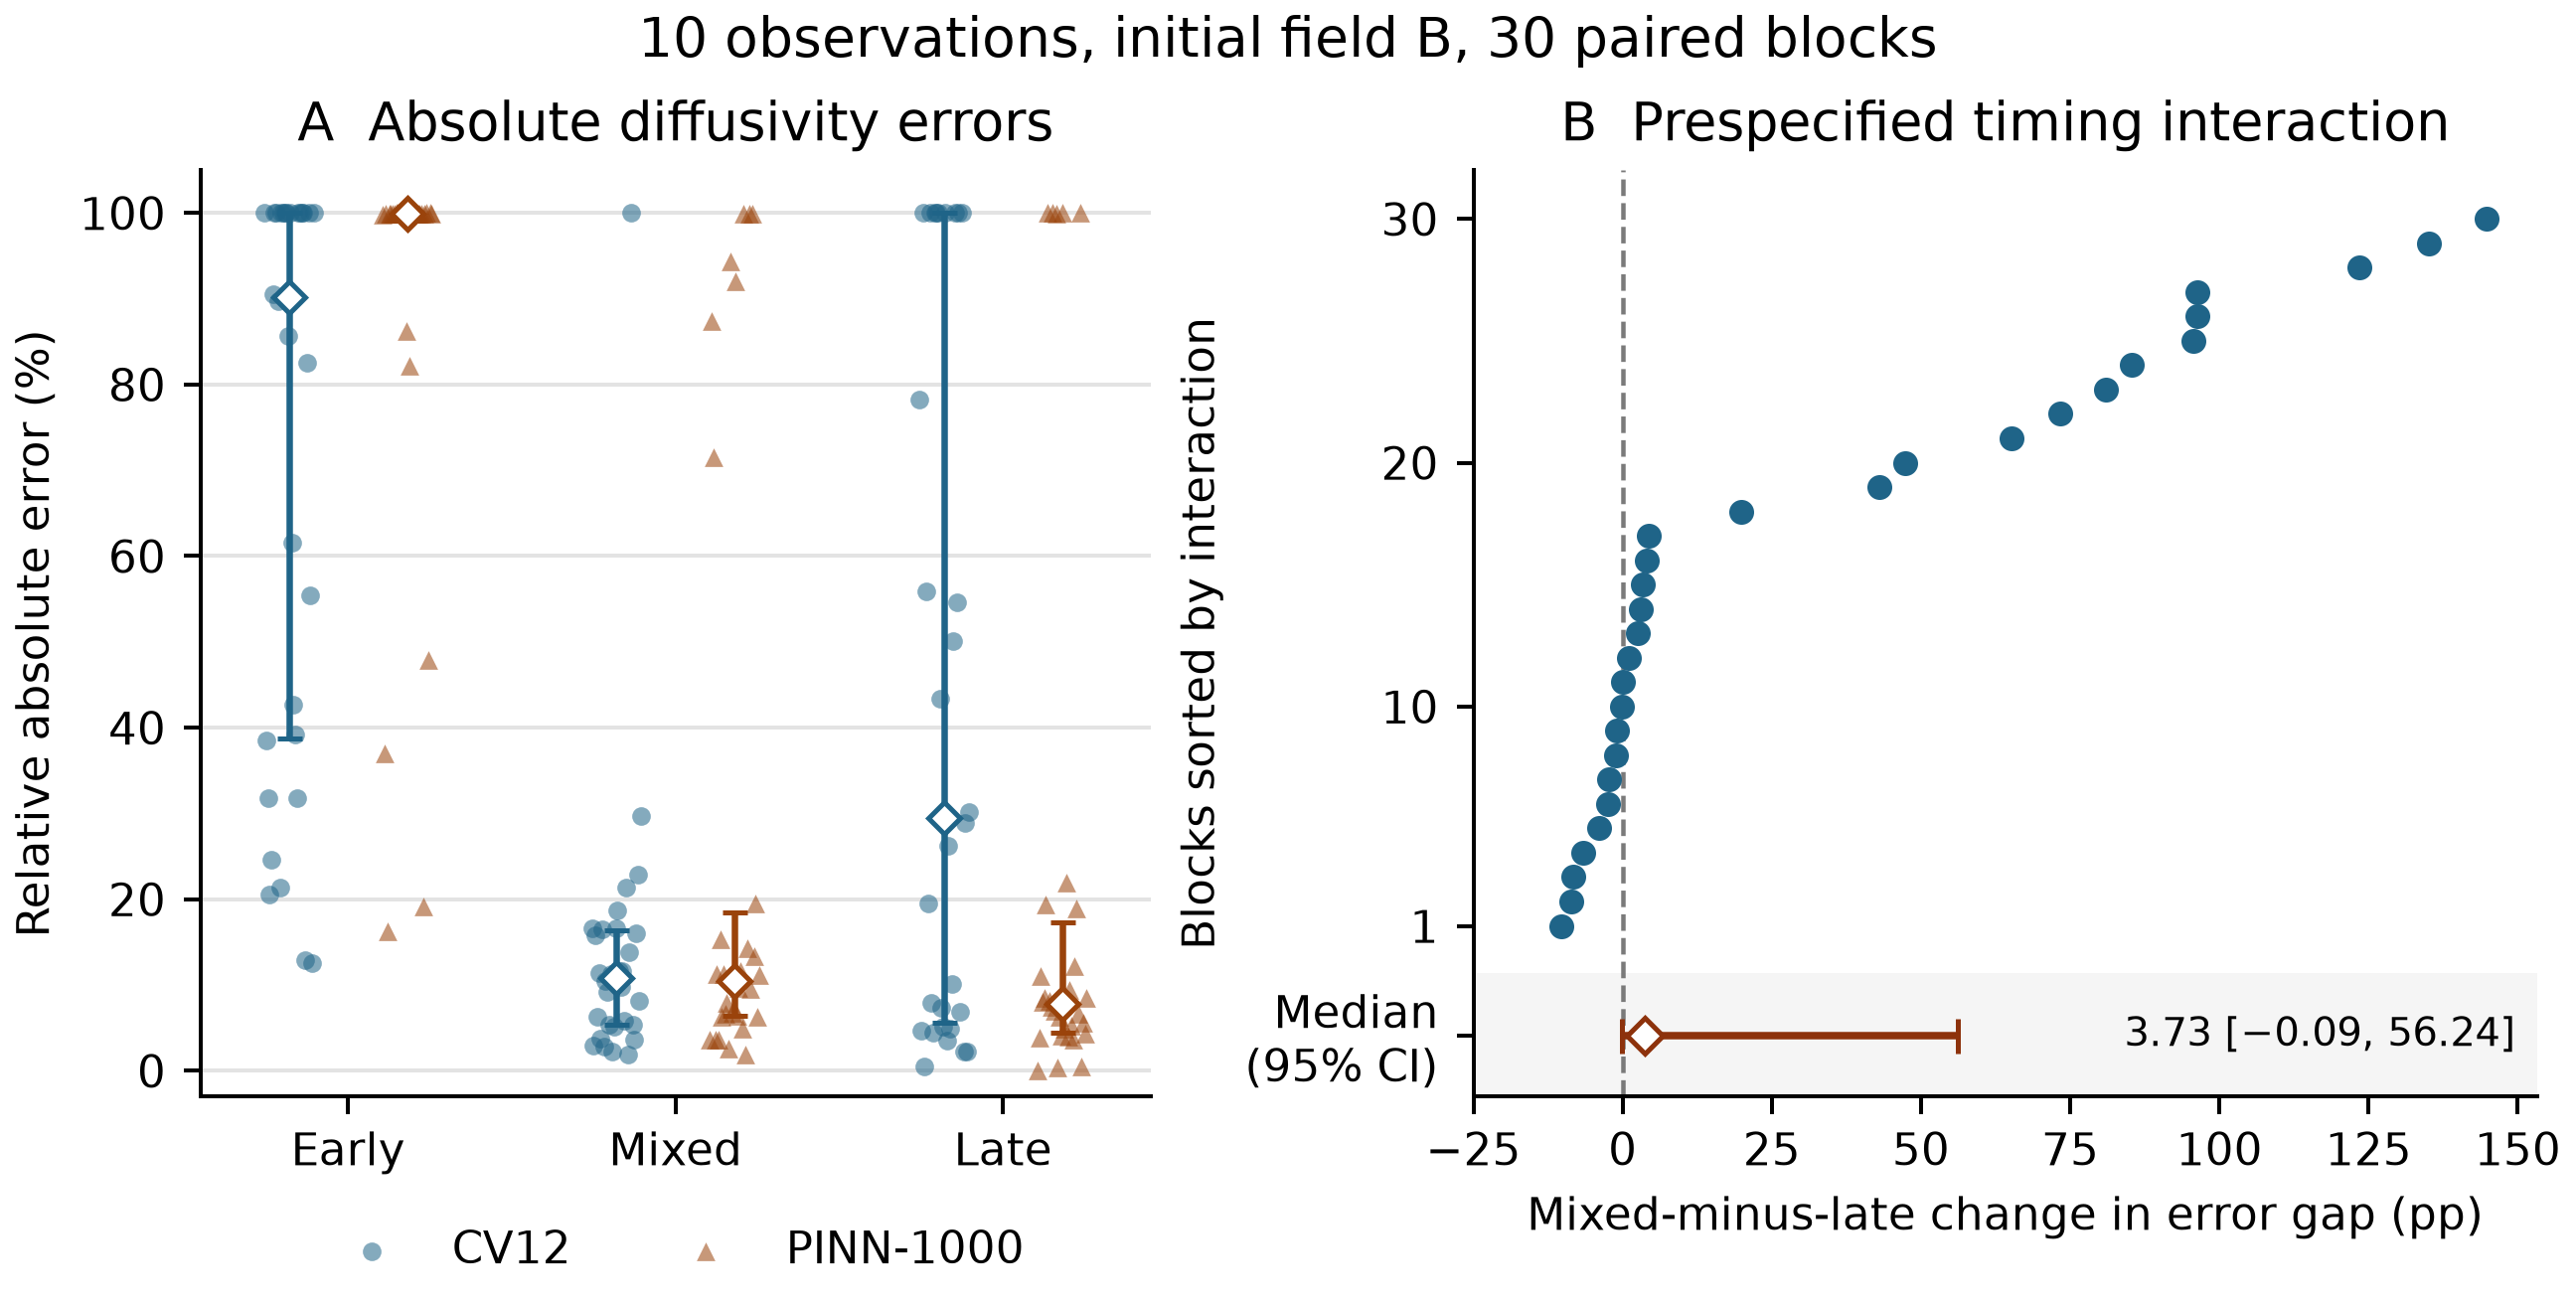
\includegraphics[width=\linewidth]{figures/primary-timing.png}
\caption{Prespecified timing result for $N=10$, field B. Panel A shows individual diffusivity errors, medians and interquartile ranges. Panel B shows the thirty blockwise mixed-minus-late interactions, their median and 95\% percentile interval from 10000 whole-block resamples. The interval spans zero.}\label{fig:timing}
\end{figure}

\subsection{What the identifiability and propagation checks show}
At $\alpha=0.05$, all thirty distinct ten-observation designs per schedule had numerical row rank ten with twelve coefficients. A and B share the matrices, so they are not additional rank replications. Equation~\eqref{eq:interpolation} explains why improved regularized recovery cannot be interpreted as restored unconstrained identifiability. At fifty observations the matrices had column rank twelve at the true diffusivity, which alone does not prove joint identification of diffusivity and coefficients.

All 720 added basis-sensitivity fits completed. For $N=50$/B with early observations, median diffusivity errors were 56.376\%, 3.528\% and 5.666\% with six, twelve and twenty-four modes. With mixed observations they were 5.880\%, 1.287\% and 1.245\%. At $N=10$/B with early observations, the corresponding values were 69.122\%, 90.130\% and 99.980\%. These contrasts show dependence on representation and regularization; they do not isolate basis dimension from the associated prior and selection rule. Profile examples are supplied in Appendix~\ref{app:profiles}.

All 360 rollout numerical screens passed after one separately archived refinement. The largest global network--rollout discrepancy was nevertheless 11.6525\%. For $N=50$/B, median discrepancies were 1.0193\% under early and 1.3491\% under mixed observations; other subgroup medians were below 0.46\%. The refined case had discrepancy 1.0410\%, with forward-refinement ratio approximately $7.0\times10^{-9}$. Passing the numerical screen establishes that the reported discrepancies are resolved by the tested refinement, not that the networks satisfy the heat equation exactly. Global norms can also conceal larger local differences.

\subsection{Localized initial field outside the twelve-mode span}
The independent truth verification found second-order spatial convergence of the finite-difference solution: maximum absolute differences were $2.25291\times10^{-4}$, $5.62948\times10^{-5}$ and $1.40732\times10^{-5}$ for 256, 512 and 1024 intervals. Observed orders were 2.0007 and 2.0000. Further spectral refinement changed the solution by less than $3\times10^{-13}$, and time-tolerance refinement by about $1.64\times10^{-9}$.

All 240 evaluation fits completed. The twelve-mode orthogonal initial projection has relative $L^2$ error 17.8605\%. Table~\ref{tab:offbasis} reports all recovery targets. Ten-observation recovery was poor for both procedures despite completion. The pointwise median paired diffusivity gaps were $-0.0234$ percentage points for mixed observations (interval $[-1.4383,7.0112]$) and $-0.2447$ for late observations (interval $[-18.7921,-0.0045]$). At fifty observations, both corresponding intervals spanned zero. The secondary mixed-minus-late interactions also spanned zero: 16.4986 percentage points, interval $[-2.3494,38.3046]$, at $N=10$, and 0.5421, interval $[-0.8181,2.2548]$, at $N=50$.

\begin{table}[htbp]\centering\small
\caption{Localized-field evaluation: marginal median percentage errors. Each condition has thirty paired blocks.}\label{tab:offbasis}
\begin{tabular}{rllrr}\toprule
$N$ & Schedule & Outcome & CV12 & PINN-1000\\\midrule
10 & mixed & diffusivity & 74.6244 & 73.0752\\
10 & mixed & initial field & 74.0456 & 70.4831\\
10 & mixed & full field & 41.8301 & 43.9698\\
10 & late & diffusivity & 99.9800 & 67.5259\\
10 & late & initial field & 82.7573 & 79.7393\\
10 & late & full field & 42.8038 & 43.8732\\
50 & mixed & diffusivity & 4.4207 & 3.3157\\
50 & mixed & initial field & 30.1281 & 24.8040\\
50 & mixed & full field & 6.9364 & 6.1261\\
50 & late & diffusivity & 7.9483 & 7.6752\\
50 & late & initial field & 65.1001 & 58.7115\\
50 & late & full field & 22.2002 & 18.7599\\
\bottomrule\end{tabular}
\end{table}


CV12 had recorded bound hits in 10 of 30 mixed and 22 of 30 late ten-observation fits; PINN-1000 had zero and one, respectively. No fifty-observation fits were flagged. Near-bound values still require inspection beyond these flags. The largest checked scoring-grid change was below 0.020 percentage points.

The large initial projection error should not be interpreted as a comparably large forward discrepancy at late sensors. A separate post-evaluation calculation propagated the exact twelve-mode orthogonal projection at the true diffusivity. The maximum absolute omitted-mode contribution over all saved late observation points was only about $2.49\times10^{-9}$, compared with noise standard deviation 0.01. Mixed observations retained larger contributions (Figure~\ref{fig:offbasis}). This diagnostic is not the fitted CV12 estimate. Field C also has initial $L^2$ norm 0.26516, different from A and B. Its changed spectrum and energy alter recovery difficulty under fixed absolute noise, so observed differences cannot be attributed exclusively to basis mismatch.

\begin{figure}[htbp]\centering
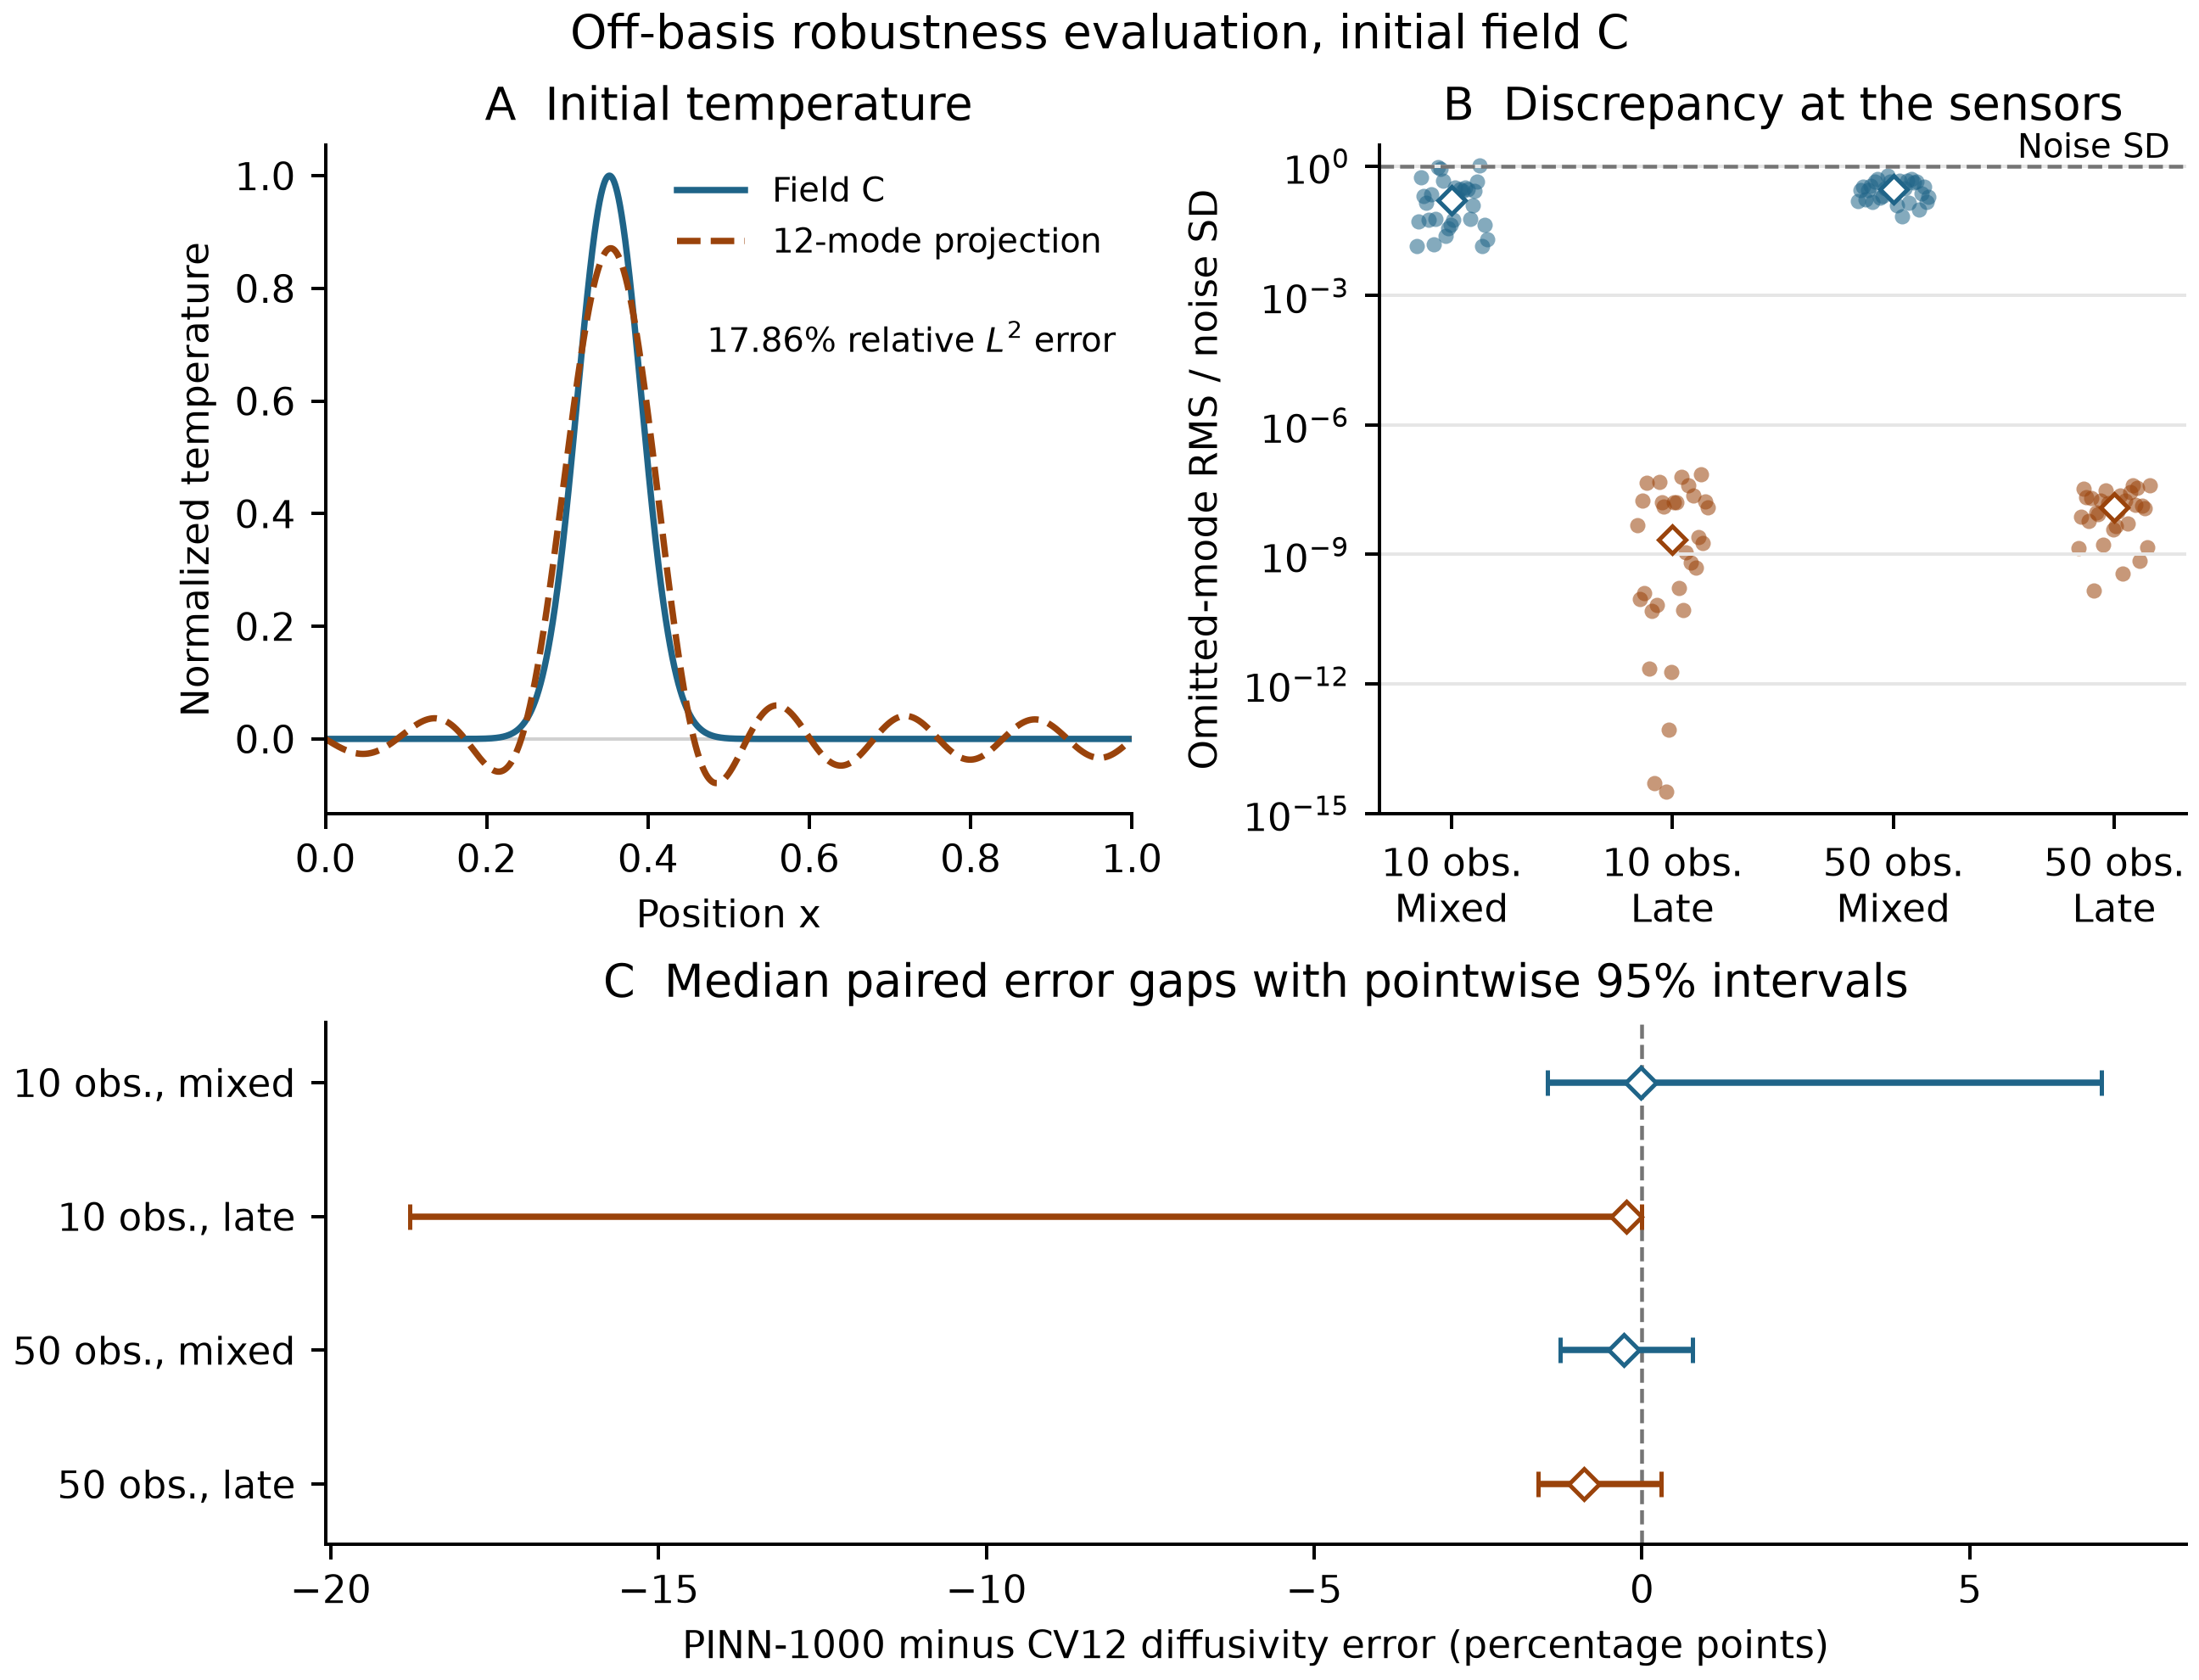
\includegraphics[width=\linewidth]{figures/offbasis.png}
\caption{Localized-field evaluation. Panel A compares the true initial field and its twelve-mode orthogonal projection. Panel B gives the omitted-mode RMS signal at observation points divided by noise standard deviation, evaluated at true diffusivity; each group contains thirty blocks. Panel C gives median paired PINN-minus-CV12 diffusivity differences with pointwise 95\% intervals. This is a secondary robustness study, not a replacement primary test.}\label{fig:offbasis}
\end{figure}

\section{Discussion}
\subsection{What survives a stronger classical baseline?}
The original comparison supports a conditional neural advantage in sparse recovery of field B even against CV12. It does not support a claim that PINNs generally defeat classical inversion. Regularization sharply improved the six-mode baseline for sparse A, and allowing twelve modes changed the denser B comparison. These controls matter because the inferred initial state is a nuisance quantity for diffusivity estimation and also a scientific target in its own right. A method can improve one target while worsening another.

The timing follow-up tests a more specific question than the original random-time study. Its primary result is uncertain, even though the schedule-level distributions and several secondary contrasts differ. Early data preserve high spatial frequencies but offer less elapsed time over which diffusion acts; delayed data encode diffusion over longer intervals while attenuating those frequencies. Unknown initial coefficients can compensate for diffusivity changes in either regime. This interpretation is consistent with the model but does not establish a causal decomposition of the measured errors into timing, optimization and regularization effects.

\subsection{Prediction, parameter recovery and physical consistency}
The rank calculation gives a concrete reason to separate regularized recovery from data-only identification. Ten scalar observations do not uniquely determine twelve unrestricted initial coefficients and diffusivity when the design matrix permits local interpolation. Good estimates can still arise from smoothness penalties, parameterization and optimization behavior. Their success is conditional on these restrictions and the tested truths.

Independent propagation asks a different question: do the quantities returned by the PINN generate its temperature trajectory under the heat equation? The answer was approximate and varied across fits. This check is useful even if parameter estimates look plausible, because a soft residual loss does not make the whole network an exact PDE solution. Conversely, perfect propagation consistency would not establish that the recovered initial state and diffusivity equal the truth.

The localized-field experiment addresses one favorable assumption of the original spectral truth. It does not remove all representation advantages or establish broad robustness. Diffusion suppressed its omitted high modes so strongly at late sensors that the initial-field projection error alone is a poor measure of forward mismatch there. A more informative account reports both initial representation error and the discrepancy at actual observation times.

\subsection{Limitations and scope of contribution}
The evidence concerns one-dimensional homogeneous diffusion, one true diffusivity, one absolute noise level, two finite spectral fields and one localized field. There are no physical measurements or unmodeled boundary effects. A known-versus-unknown initial-temperature control, multiple diffusivities and noise levels, and equal tuning budgets were not performed. They are possible future studies, not missing results filled by inference.

Thirty independent blocks per observation count improve the follow-up design relative to the original ten, but do not guarantee precise bootstrap intervals, particularly near parameter bounds. Most reported intervals are secondary and unadjusted. The original neural summaries use three starts whereas the follow-ups use one start, preventing an initialization-independent conclusion. The expanded ridge grid also distinguishes the follow-ups from the original baseline. The rank and rollout checks were introduced after evaluation and must not be described as preregistered.

The contribution is an empirical assessment of specified inversion procedures under controlled changes in regularization, initial-state representation, optimization budget and observation timing. Existing work establishes joint heat inversion, neural initial-state recovery and the role of initial conditions in identifiability \citep{ref002,ref003,ref076,bilo2026}. The present audit links paired recovery errors to finite-sample interpolation, sensitivity to regularization and basis size, and independent propagation of learned quantities. The original comparison supplies the baseline evidence, the timing evaluation tests the added measurement question, and the localized field examines dependence on finite-mode truths. Unresolved and unfavorable results remain part of that assessment.

\section{Conclusion}
Regularization, initial-state representation and measurement schedule materially affect the interpretation of this heat-inversion comparison. The original sparse field-B result favored the longer-budget PINN on several outcomes, while denser data favored CV12 for full-field recovery. The prespecified timing interaction remained unresolved. Full-row-rank interpolation explains why improved sparse regularized estimates do not establish unconstrained identifiability, and independent propagation revealed nonzero physical inconsistency in saved PINNs. The localized-field evaluation extended the empirical scope while exposing the distinction between time-zero representation error and forward discrepancy at delayed sensors. These findings support reporting specified procedures, separate recovery targets and uncertainty rather than assigning a general ranking to PINNs and classical methods.

\section*{Declarations}
\textbf{Funding.} This research received no funding.

\noindent\textbf{Competing interests.} The author declares no competing interests.

\noindent\textbf{Author contribution.} Ridoy Hasan is the sole author and is responsible for the research and manuscript.

\noindent\textbf{AI assistance.} Claude and ChatGPT assisted with developing and debugging experimental and analysis code. ChatGPT also assisted with literature searching, manuscript drafting and revision, and preparation of the submission files. Numerical results reported here come from the archived computational experiments. Responsibility for checking the sources, interpretations and final submitted text rests with the author; AI tools are not authors.

\noindent\textbf{Research materials.} The study uses synthetic observations of a mathematical model; no human participant or animal data were collected.

\noindent\textbf{Data and code availability.} Code, protocols and analysis are available at \url{https://github.com/ridoy1211/pinn-audit}. The original experiment archive is preserved at commit \texttt{4a64ed4cae0991bb957c18dd2bcea26162bd4e22}. Timing, explanatory diagnostics and localized-field evidence are available in the release \href{https://github.com/ridoy1211/pinn-audit/releases/tag/heat-inversion-evidence-v1.0.0}{\texttt{heat-inversion-evidence-v1.0.0}}. The \texttt{experiment/controlled-timing} branch contains follow-up reporting and restoration tools. Historical frozen records distinguish evaluation sources from later documentation and reporting changes.

\FloatBarrier
\clearpage
\appendix
\section{Original comparison tables}\label{app:original}
\small
\begin{longtable}{rllrrr}
\caption{Original comparison: marginal median errors (\%). Each neural score first takes the median over three starts, separately for each outcome; each stratum contains ten designs.}\label{tab:original}\\
\toprule
$N$ & Field & Procedure & $E_\alpha$ & $E_u$ & $E_f$\\\midrule
\endfirsthead
\toprule
$N$ & Field & Procedure & $E_\alpha$ & $E_u$ & $E_f$\\\midrule
\endhead
10 & A & unreg6 & 9.259 & 10.242 & 37.274\\
10 & A & fixed6 & 4.030 & 3.439 & 8.508\\
10 & A & CV6 & 4.030 & 3.439 & 8.508\\
10 & A & CV12 & 4.755 & 3.942 & 10.900\\
10 & A & PINN-200 & 3.919 & 3.717 & 8.803\\
10 & A & PINN-1000 & 2.580 & 3.842 & 8.963\\
10 & B & unreg6 & 9.268 & 12.976 & 51.270\\
10 & B & fixed6 & 6.343 & 6.187 & 24.206\\
10 & B & CV6 & 7.550 & 6.278 & 24.206\\
10 & B & CV12 & 11.752 & 7.402 & 26.111\\
10 & B & PINN-200 & 9.205 & 6.040 & 23.810\\
10 & B & PINN-1000 & 3.400 & 6.071 & 23.368\\
50 & A & unreg6 & 1.325 & 0.862 & 2.473\\
50 & A & fixed6 & 1.326 & 0.834 & 2.064\\
50 & A & CV6 & 1.420 & 0.834 & 2.064\\
50 & A & CV12 & 1.607 & 0.889 & 2.919\\
50 & A & PINN-200 & 1.402 & 0.760 & 1.573\\
50 & A & PINN-1000 & 1.494 & 0.909 & 2.366\\
50 & B & unreg6 & 3.625 & 5.899 & 26.250\\
50 & B & fixed6 & 3.761 & 5.218 & 23.362\\
50 & B & CV6 & 5.526 & 6.233 & 24.982\\
50 & B & CV12 & 1.902 & 2.191 & 10.882\\
50 & B & PINN-200 & 5.356 & 4.933 & 22.352\\
50 & B & PINN-1000 & 2.334 & 3.703 & 16.482\\
\bottomrule
\end{longtable}
\normalsize
\small
\begin{longtable}{rlllrlr}
\caption{Original comparison: all planned paired PINN-minus-CV12 contrasts in percentage points. Intervals are pointwise 95\% percentile bootstrap intervals over ten designs. W/T/L counts strict neural wins, ties and losses.}\label{tab:originalpaired}\\
\toprule
$N$ & Field & PINN budget & Outcome & Median & Interval & W/T/L\\\midrule
\endfirsthead
\toprule
$N$ & Field & PINN budget & Outcome & Median & Interval & W/T/L\\\midrule
\endhead
10 & A & 200 & diffusivity & +0.078 & [-12.210, 2.788] & 5/0/5\\
10 & A & 200 & field & +0.072 & [-3.303, 1.391] & 4/0/6\\
10 & A & 200 & initial field & +0.420 & [-8.141, 3.834] & 4/0/6\\
10 & A & 1000 & diffusivity & -0.135 & [-11.756, 0.895] & 6/0/4\\
10 & A & 1000 & field & -0.382 & [-2.983, 0.661] & 6/0/4\\
10 & A & 1000 & initial field & -0.766 & [-7.597, 2.538] & 6/0/4\\
10 & B & 200 & diffusivity & -1.333 & [-14.067, 3.610] & 6/0/4\\
10 & B & 200 & field & -0.527 & [-2.774, 1.585] & 6/0/4\\
10 & B & 200 & initial field & -0.743 & [-4.046, 2.201] & 6/0/4\\
10 & B & 1000 & diffusivity & -4.445 & [-22.168, -1.109] & 9/0/1\\
10 & B & 1000 & field & -1.117 & [-3.099, -0.136] & 8/0/2\\
10 & B & 1000 & initial field & -1.508 & [-5.148, -0.467] & 9/0/1\\
50 & A & 200 & diffusivity & +0.059 & [-0.597, 1.016] & 4/0/6\\
50 & A & 200 & field & -0.058 & [-0.261, 0.019] & 6/0/4\\
50 & A & 200 & initial field & -0.694 & [-1.543, -0.216] & 9/0/1\\
50 & A & 1000 & diffusivity & +0.042 & [-0.643, 0.878] & 5/0/5\\
50 & A & 1000 & field & +0.055 & [-0.049, 0.269] & 3/0/7\\
50 & A & 1000 & initial field & -0.024 & [-0.516, 0.884] & 5/0/5\\
50 & B & 200 & diffusivity & +2.031 & [1.209, 4.901] & 1/0/9\\
50 & B & 200 & field & +2.862 & [2.021, 3.562] & 0/0/10\\
50 & B & 200 & initial field & +11.866 & [7.869, 15.369] & 0/0/10\\
50 & B & 1000 & diffusivity & +0.410 & [-0.386, 1.616] & 4/0/6\\
50 & B & 1000 & field & +0.803 & [0.032, 2.142] & 2/0/8\\
50 & B & 1000 & initial field & +2.577 & [-0.303, 11.081] & 3/0/7\\
\bottomrule
\end{longtable}
\normalsize
\begin{table}[htbp]\centering\small
\caption{Original median computation times (seconds). CV12 includes selection and the selected fit; each neural entry sums training time for three starts. Evaluation is excluded. This is not an equal-compute comparison.}\label{tab:cost}
\begin{tabular}{rlrrr}\toprule
$N$ & Field & CV12 & PINN-200 & PINN-1000\\\midrule
10 & A & 7.25 & 73.91 & 115.24\\
10 & B & 9.56 & 83.70 & 121.64\\
50 & A & 11.05 & 88.67 & 124.17\\
50 & B & 10.40 & 95.01 & 121.62\\
\bottomrule\end{tabular}
\end{table}

\FloatBarrier
\section{Additional timing outcomes}
Initial-field and full-field errors remain distinct from diffusivity errors. The following marginal summaries do not provide paired effect estimates; the complete paired tables and pointwise intervals are archived with the timing analysis.
\begin{table}[htbp]\centering\small
\caption{Timing evaluation: marginal median initial-field and full-field errors (\%).}\label{tab:fields}
\begin{tabular}{rllrrrr}\toprule
$N$ & Field & Schedule & $E_f$, CV12 & $E_f$, PINN & $E_u$, CV12 & $E_u$, PINN\\\midrule
10 & A & early & 8.170 & 11.423 & 8.660 & 44.127\\
10 & A & mixed & 6.167 & 4.983 & 2.557 & 2.538\\
10 & A & late & 20.823 & 14.561 & 8.300 & 5.552\\
10 & B & early & 20.945 & 24.060 & 40.484 & 47.799\\
10 & B & mixed & 22.108 & 22.891 & 5.584 & 6.097\\
10 & B & late & 29.820 & 25.307 & 9.390 & 6.831\\
50 & A & early & 1.751 & 1.141 & 1.355 & 1.343\\
50 & A & mixed & 2.027 & 1.496 & 0.683 & 0.581\\
50 & A & late & 4.102 & 4.514 & 1.564 & 1.488\\
50 & B & early & 3.586 & 4.435 & 1.145 & 1.580\\
50 & B & mixed & 4.725 & 5.468 & 1.025 & 1.009\\
50 & B & late & 22.188 & 22.201 & 4.674 & 4.671\\
\bottomrule\end{tabular}
\end{table}

\FloatBarrier
\clearpage
\section{Explanatory profiles and independent propagation}\label{app:profiles}
\begin{figure}[htbp]\centering
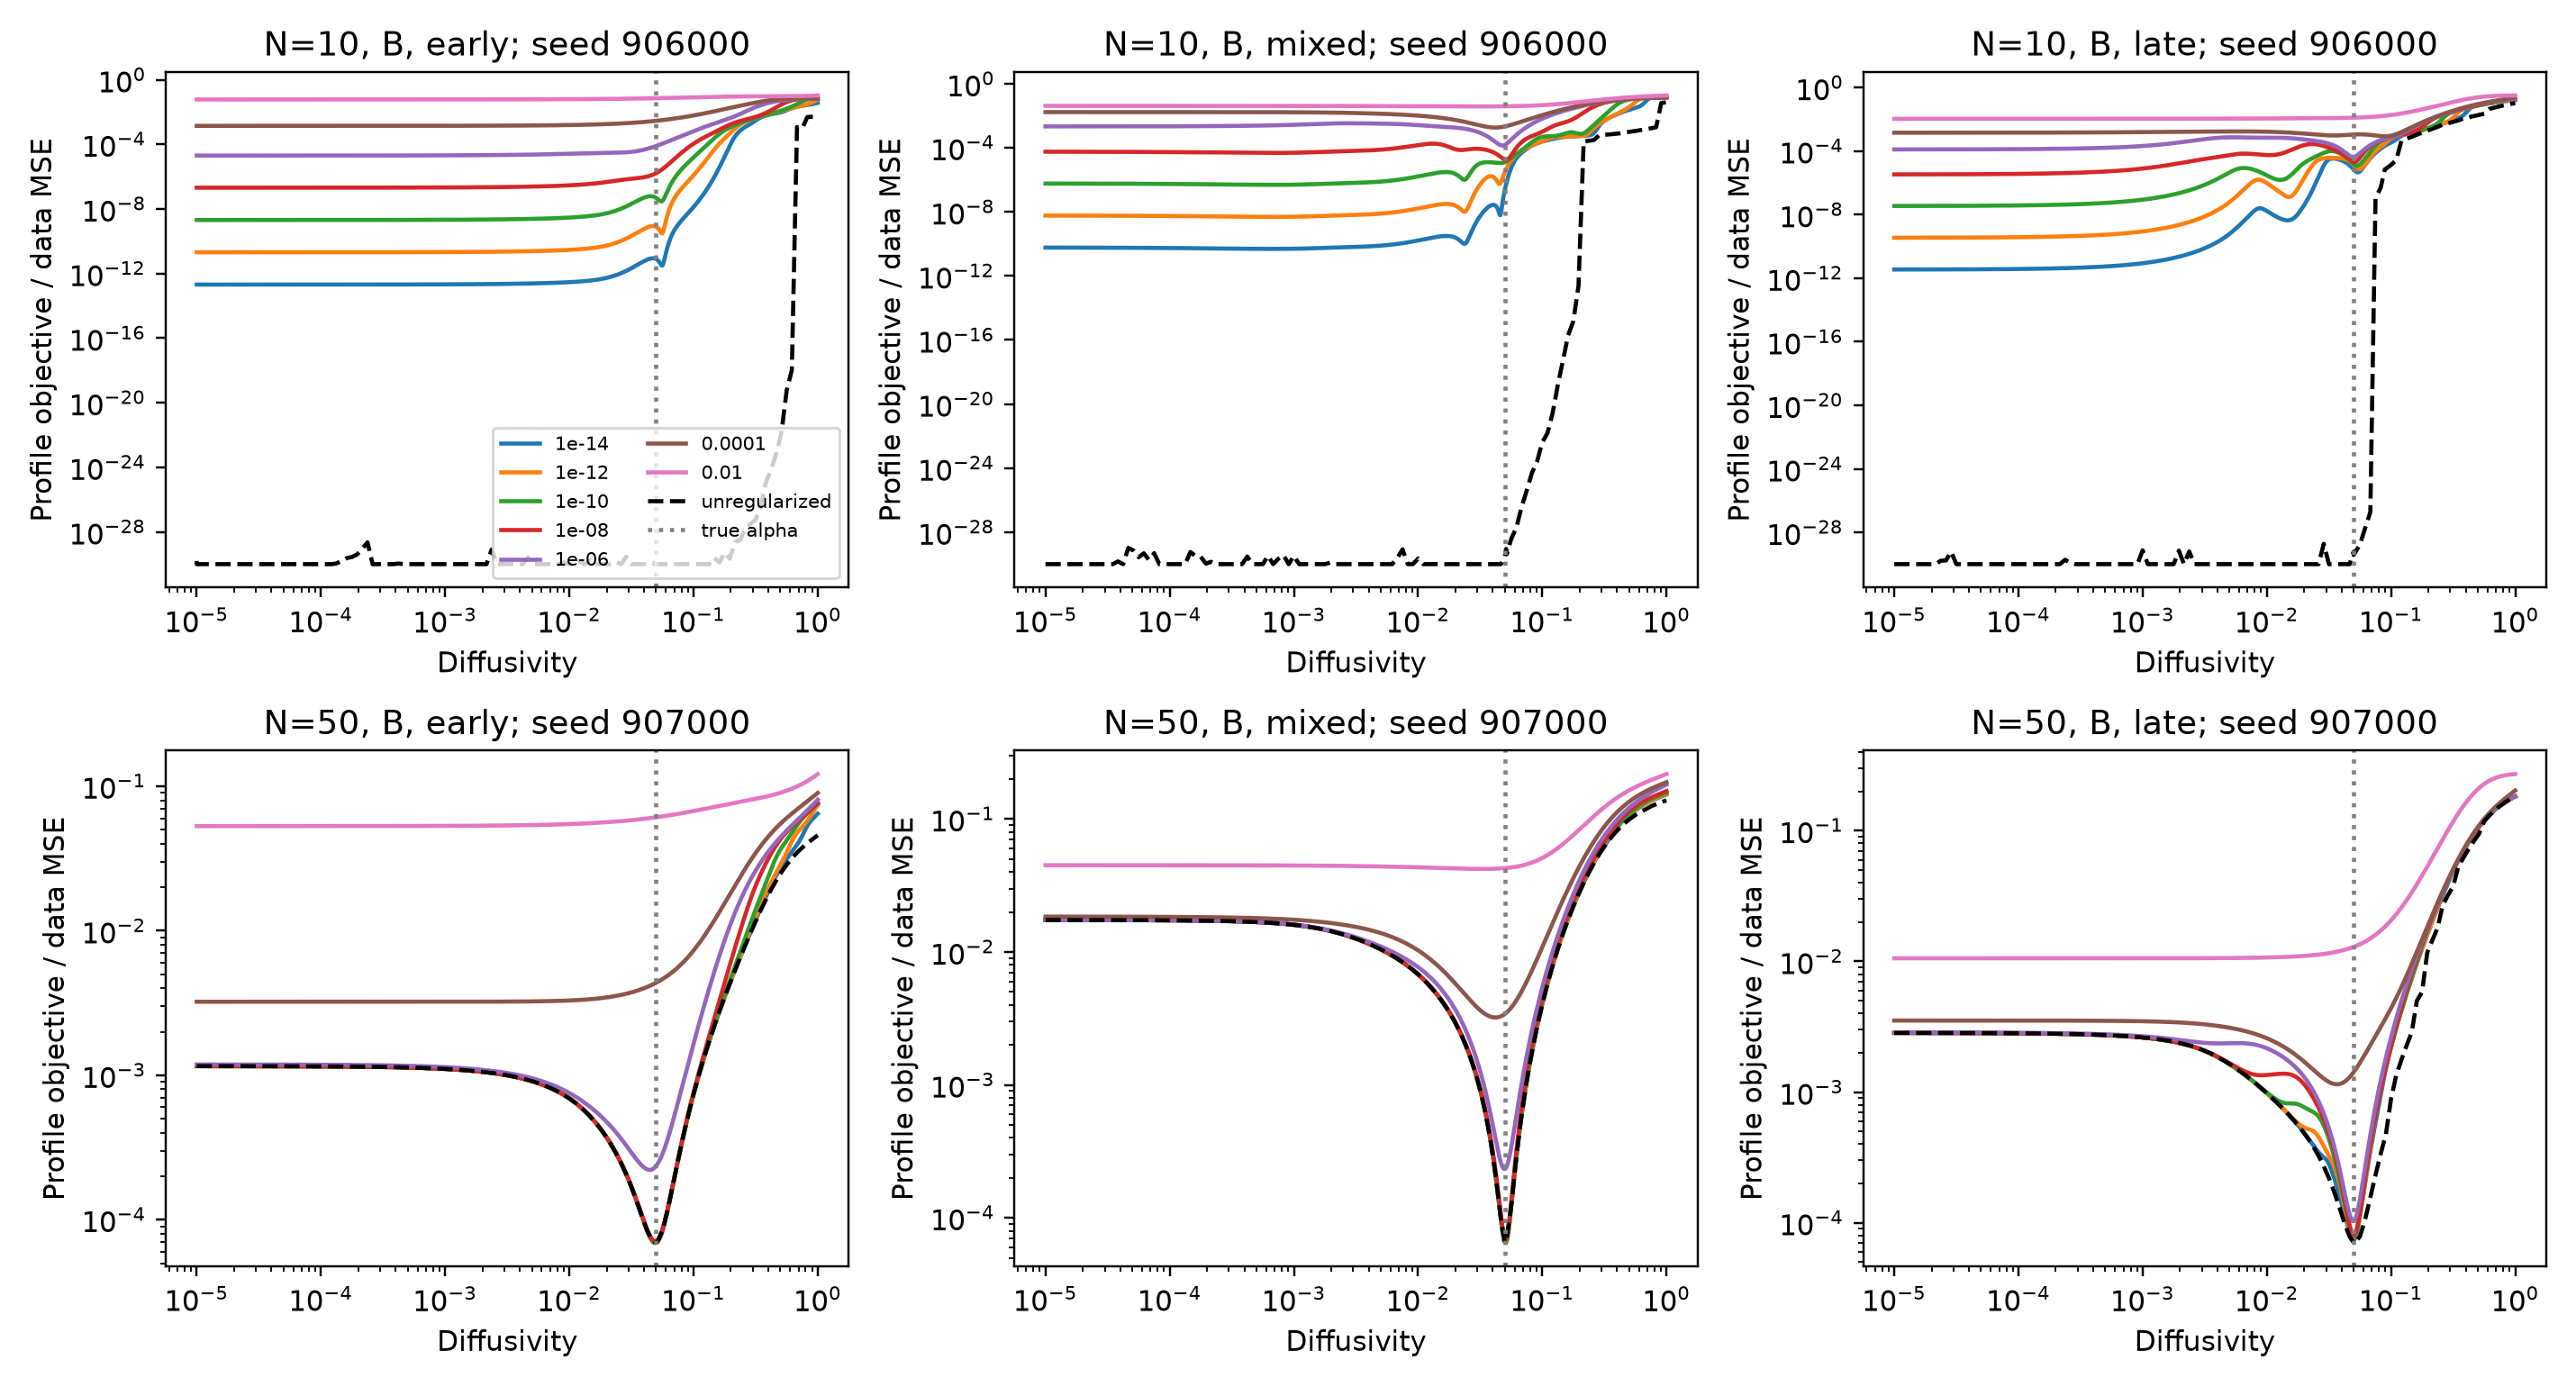
\includegraphics[width=\linewidth]{figures/profiles.png}
\caption{Post-evaluation profiles for field B and the first evaluation seed at each observation count, across all schedules. Initial coefficients are refitted at each diffusivity. Seed order, not error, selects the examples. Positive-penalty curves are different objectives and must not be ranked vertically to choose a penalty. Zero values are floored at $10^{-30}$ for plotting.}\label{fig:profiles}
\end{figure}
\begin{figure}[htbp]\centering
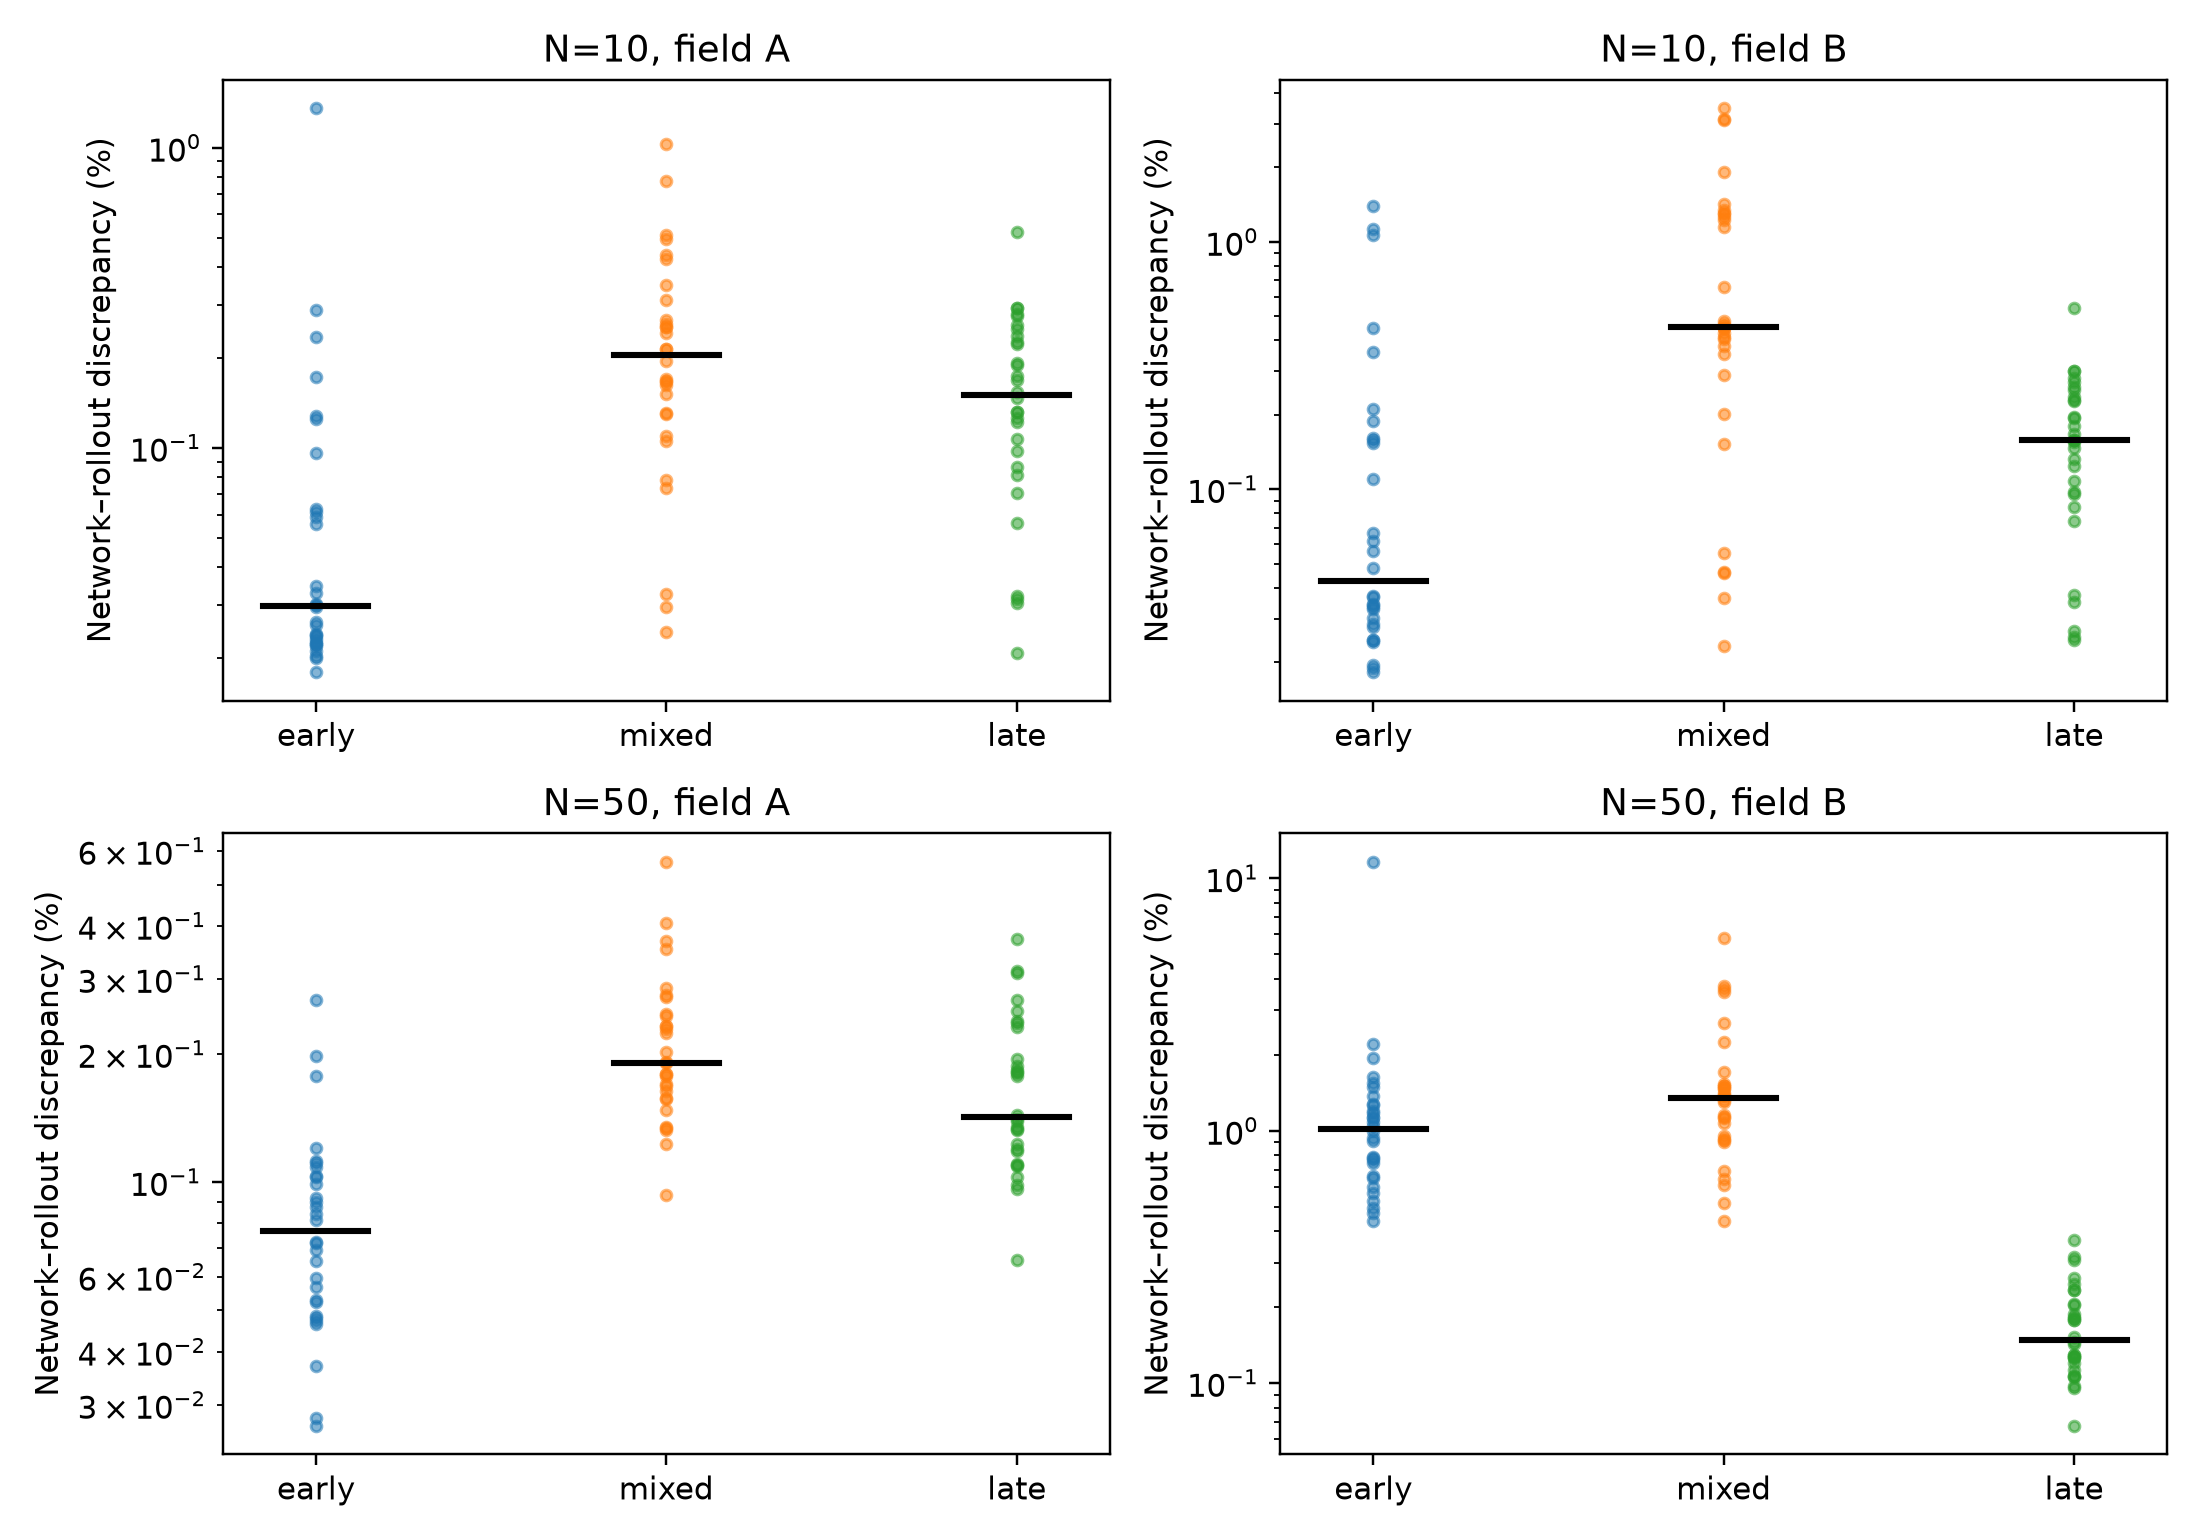
\includegraphics[width=\linewidth]{figures/physical-consistency.png}
\caption{Independent propagation discrepancy for all 360 timing PINNs after the separately recorded refinement. Each point uses the learned initial field and diffusivity. Black marks show subgroup medians. Numerical refinement screens passing does not imply physical exactness or accurate recovery against truth.}\label{fig:rollout}
\end{figure}
\FloatBarrier
\bibliographystyle{unsrtnat}
\bibliography{references}
\end{document}
